%%%%%%%%%%%%%%%%%%%%%%%%%%%%%%%%%%%%%%%%%%%%%%%%%%%%%%%%
\fondo{celeste}
\section{GPTs para errores intencionados}
\fondo{blanco}
%%%%%%%%%%%%%%%%%%%%%%%%%%%%%%%%%%%%%%%%%%%%%%%%%%%%%%%%

\begin{frame}
    \frametitle{La IA mejora: menos alucinaciones}

    \centering
    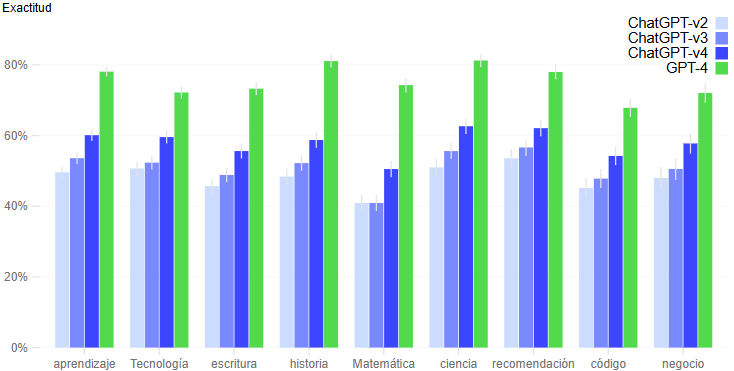
\includegraphics[width=0.85\linewidth]{Figuras/Fig10.png}
\end{frame}


\begin{frame}
    \frametitle{¿Y si la IA ya no alucina?}

    \begin{itemize}
         \item Modelos recientes, como \textbf{GPT-4}, muestran una mejora significativa en la exactitud de sus respuestas.
        \item Esta mejora \textbf{reduce las alucinaciones}, pero también limita los casos espontáneos útiles para el aprendizaje crítico.
        \item \textbf{¿Cómo conservar el valor didáctico de las alucinaciones si la IA deja de cometerlas?}
    \end{itemize}
\end{frame}


\begin{frame}

     Se creó un GPT personalizado llamado  \href{https://chatgpt.com/g/g-6853670f47648191917d013f9d97448c-derivador-3000}{\textbf{Derivador 3000}}.

    \centering
    \postitimg[0.8\linewidth]{Figuras/Fig12.png}\\\footnotesize
    \url{https://chatgpt.com/g/g-6853670f47648191917d013f9d97448c-derivador-3000}
\end{frame}

\begin{frame}


    Está diseñado para cometer \textbf{errores sutiles y esporádicos} en derivación.


    \centering
    \postitimg[0.85\linewidth]{Figuras/Fig13.png}
\end{frame}

